\documentclass{article}
\usepackage{amsmath, amscd, amssymb, amsthm, latexsym}
\usepackage[spanish]{babel}
\usepackage{enumerate}
\usepackage{float}
\usepackage[table]{xcolor}
\usepackage{geometry}
\usepackage{url}
\usepackage{booktabs}
\usepackage{tabularx}
\usepackage{graphicx}
\usepackage{caption}
\usepackage{hyperref}
\usepackage{graphics}
\usepackage{algorithm, algpseudocode}
\usepackage{tikz}

\graphicspath{{img/}}

\hypersetup{
  colorlinks=true,
  linkcolor=blue!80!red,
  urlcolor=green!70!black
}


\newcommand{\BigO}[1]{{\mathcal{O}(#1)}}
\newcommand{\BigOmega}[1]{{\Omega(#1)}}
\newcommand{\BigTheta}[1]{{\Theta(#1)}}
\newcommand{\code}{\texttt}

\newtheorem*{theorem*}{Teorema}


\title{Resumen para Algoritmos y Estructuras de Datos II}
\author{Tomás Spognardi}
\date{\today}

\begin{document}

\maketitle

\tableofcontents

\newpage

\section{Tipos Abstractos de Datos}

Un \textit{Tipo Abstracto de Datos} (TAD) está definido por un \textbf{tipo}, es decir, un conjunto de valores y operaciones entre los mismos, y la \textbf{semántica} de esas operaciones (en este caso, se describe a través de \textbf{axiomas}).

Los TADs se diseñan a partir de la especificación informal de un problema. Un paso importante es el de \textbf{abstracción}, que consiste en identificar los aspectos importantes del problema e ignorar el resto de los detalles.

Por otro lado, un TAD no especifica ninguna implementación del comportamiento que describe: delinea el qué, y no el cómo.

Formalmente, cada TAD define una teoría de primer orden con igualdad. Esto se logra especificando la \textbf{signatura} de las operaciones, junto con la cual se definen \textbf{restricciones} sobre el dominio de cada una, y los \textbf{axiomas} que cumplen.

\subsection{Secciones de un TAD}

Las siguientes son las posibles secciones incluidas en la definición de un TAD.
\begin{itemize}
    \item \textbf{Parámetros formales:} Son los tipos y operaciones requiridas por los TADs paramétricos.
    \item \textbf{Igualdad Observacional:} Define el criterio bajo el cuál las instancias de un TAD son indistinguibles.
    \item \textbf{Género:} Es el nombre que recibe el conjunto de valores del tipo.
    \item \textbf{Usa:} Incluye los géneros y operaciones externas con las que interactúa el TAD.
    \item \textbf{Exporta:} Las operaciones y géneros que quedan a disposición de usuarios del tipo.
    \item \textbf{Generadores:} Son las operaciones que permiten construir valores del tipo. Para ser adecuadas, debe ser posible construir cualquier instancia posible a través de ellas. Además, es ideal que sean \textit{minimales}, es decir, el conjunto más chico posible que cumple la condición anterior.
    \item \textbf{Observadores Básicos:} Son las operaciones que permiten obtener información acerca de las instancias de un tipo. También es conveniente que sean minimales.
    \item \textbf{Otras Operaciones:} Las operaciones que no son generadores ni observadores.
    \item \textbf{Axiomas:} Son las reglas que definen el comportamiento de las funciones.
\end{itemize}

\subsection{Errores de especificación}

\begin{itemize}
    \item \textbf{Sobreespecificación:} La sobreespecificación se da cuando varios axiomas aplican a la misma instancia, lo cual causa inconsistencias lógicas. Para evitarla, es importante recordar que los TADs no admiten ``pattern matching'': el orden de los axiomas no tiene ningún efecto sobre su aplicación.
    \item \textbf{Subespecificación:} Implica no definir axiomas sobre el comportamiento de una operación para ciertas instancias del tipo. No siempre es un problema, como en el caso de \textit{dameUno} del TAD \textsc{CONJUNTO}.
    \item \textbf{Casos Restringidos:} Los axiomas no deben especificar sobre casos restringidos, ya que están fuera del dominio.
    \item \textbf{Incongruencia:} Se da cuando una de las operaciones de un TAD no es \textit{congruente}\footnote{Una función $f$ es congruente con respecto a una relación de equivalencia $\sim$ cuando $\forall x, y,\ \ x \sim y \Longleftrightarrow f(x) \sim f(y) $} con respecto a la igualdad observacional, es decir, se vuelve posible diferenciar elementos dentro de la misma clase de equivalencia de esta relación.
\end{itemize}

Una buena práctica para evitar errores es axiomatizar los observadores básicos sobre todos los generadores no restringidos, y definir las otras operaciones utilizándolos. De esta forma se puede garantizar la congruencia con respecto a la igualdad observacional.

\subsection{Igualdad observacional}

La \textbf{igualdad observacional} es un predicado binario entre las instancias de un tipo que indica cuándo son iguales. Es parte del metalenguaje, y como tal no puede ser utilizado dentro de los axiomas. Generalmente, se define en términos de los observadores básicos.

Cuando dos instancias son observacionalmente iguales, se los considera indistinguibles, así que cualquier operación aplicada a ambos debe tener el mismo resultado. Esto puede servir como criterio para definir los observadores básicos: se busca el conjunto minimal de operaciones que permita diferenciar entre todas las instancias de un tipo.

\section{Complejidad Computacional}

La complejidad computacional es una medida de la eficiencia de un algoritmo en términos de su consumo de recursos, y permite comparar algoritmos entre sí. Los recursos considerados incluyen:
\begin{itemize}
    \item Tiempo de ejecución.
    \item Espacio en memoria.
    \item Cantidad de proceasadores.
    \item Utilización de la red de comunicaciones.
\end{itemize}

El análisis de complejidad se puede realizar de dos formas distintas:

\begin{itemize}
    \item \textbf{Empírica:} Es el método más primitivo, y consiste en medir los recursos utilizados por una computadora particular en un conjunto de entradas concreto (idealmente, representativo de las entradas sobre las cuales se va a implementar). Tiene la desventajas de no ser portable y potencialmente consumir mucho tiempo.
    \item \textbf{Teórica:} Se basa en un análisis estático del algoritmo dado un modelo de cómputo, sin necesidad de implementarlo ni correrlo. Es independiente de la máquina y lenguaje de programación, y vale para todas las instancias del problema. Es el método que utilizamos en la cursada.
\end{itemize}

El análisis teórico de la complejidad computacional se basa en un modelo de cómputo consensuado, y en general se hace en función del tamaño del input. Si hay características de las entradas que causan variaciones importantes en el consumo de recursos, entonces se pueden analizar como distintos tipos de input. Por último, se realiza un análisis del comportamiento asintótico, es decir, el crecimiento de la función a medida que se toman instancias de mayor tamaño.

\subsection{Modelo de cómputo}

Formalmente, un modelo de cómputo define la forma en la que una función matemática es computada dada una entrada. En este caso se utiliza para definir qué operaciones pueden ser realizadas en un tiempo acotado por una constante $c$, llamadas \textit{Operaciones Elementales} (OE).

Consideramos OEs a las operaciones aritméticas básicas, las operaciones lógicas, las transferencias de control, y asignaciones de variables a tipos básicos. Para contar la cantidad de OEs que realizan las estructuras de control de flujo, se pueden utilizar las siguientes reglas generales:
\begin{itemize}
    \item Condiciones:
          $$T(\code{if $C$ then $S_1$ else $S_1$ end}) = T(C) + \max{\{T(S_1), T(S_2)\}}$$
    \item Loops:
          $$T(\code{while $C$ do $S$ end}) = T(C) + \text{\#iteraciones} \cdot (T(S) + T(C))$$
    \item Llamadas:
          $$T(F(P_1, P_2, P_n)) = 1 + \sum_{i = 1}^n T(P_i) + T(F)$$
\end{itemize}

El resto de las estructuras (\code{for}, \code{switch}, etc.) pueden ser reescritas en términos de las anteriores. Se debe tener en cuenta que esto da una cota superior de la cantidad de operaciones realizadas, y a veces se requiere un análisis más profundo (en especial en el caso de \code{if}).

\subsection{Cantidad de operaciones elementales}

Luego, para cada algoritmo $A$, se define la función $t_A: I_A \Rightarrow \mathbb{N}$, donde $t_A(I)$ indica la cantidad de operaciones elementales que realiza el algoritmo $A$ para la entrada $I \in I_A$. Luego, si se toma $T_A(I)$ como el tiempo que tarda $A$ en ser ejecutado para la instancia $I$, se tiene que:
$$ T_A(I) \leq c \cdot t_A(I) $$

Esta definición permite comparar el tiempo de ejecución entre distintos algoritmos al contar la cantidad de operaciones elementales que realizan. Más aún, vamos a tomar como unidad de tiempo a la constante $c$, por lo cual cada OE tomará a lo sumo una unidad de tiempo (y por conveniencia, definimos $T(OE) = 1$, ya que es indistinto a la hora de hacer análisis asintótico).

\subsection{Tamaño de la entrada}

Considerar la complejidad en función del tamaño de una entrada, en cambio de la entrada en sí, simplifica el análisis. Sin embargo, es posible que distintas instancias del mismo tamaño consuman distintas cantidades de recursos. Para remediar esto, suelen estudiarse tres casos para cada algoritmo:

\begin{itemize}
    \item \textbf{Caso peor:} Es la medida que más se usa, porque asegura garantías certeras (aunque pesimistas) sobre el tiempo de ejecución de un algoritmos. Se define como:
          $$T_{\text{peor}}(n) = \max{\{t(i)} \mid I \in I_A, |I| = n\}$$
    \item \textbf{Caso mejor:} Es dual al caso peor, dado que se define como:
          $$T_{\text{mejor}}(n) = \min{\{t(i)} \mid I \in I_A, |I| = n\}$$
    \item \textbf{Caso promedio:} Intuitivamente $T_{\text{prom}}(n)$ se corresponde al ``tiempo esperado'' sobre instancias típicas. Definirla requiere conocer la distribución estadística del input, que en muchos casos no es posible. Si $P(I)$ es la probabilidad de que el input sea la instancia $I$, entonces está definida por:
          $$T_{\text{prom}}(n) = \sum_{I \in I_A, |I| = n} P(I) \cdot t(I) $$
\end{itemize}

\subsection{Análisis asintótico}

El \textit{orden} de la función $T(n)$ es el que expresa el comportamiento dominante cuando el tamaño de la entrada es grande. Existen distintas medidas para analizarlo:

\begin{itemize}
    \item $\mathcal{O}$, la cota superior.
    \item $\Omega$, la cota inferior.
    \item $\Theta$, el orden exacto.
\end{itemize}

\subsubsection{Cota superior}

Se define como:
$$\BigO{f} = \{ g \mid \exists n_0, k > 0 \text{ tal que } \forall n \geq n_0,\ g(n) \leq k \cdot f(n) \}$$

Es decir, $g \in \BigO{f}$ significa que, asintóticamente, $g$ no crece más que $f$.

La cota superior permite obtener una garantía sobre el comportamiento asintótico de una función, y cumple las siguientes propiedades:
\begin{enumerate}
    \item $f \in \BigO{f}$
    \item $f \in \BigO{g} \implies \BigO{f} \subseteq \BigO{g}$
    \item $\BigO{f} = \BigO{g} \iff f \in \BigO{g} \land g \in \BigO{f}$
    \item $f \in \BigO{g} \land g \in \BigO{h} \implies f \in \BigO{h}$
    \item $f \in \BigO{g} \land f \in \BigO{h} \implies f \in \BigO{\min{\{g, h\}}}$
    \item $f_1 \in \BigO{g} \land f_2 \in \BigO{h} \implies f_1 + f_2 \in \BigO{\max{\{g, h\}}}$
    \item $f_1 \in \BigO{g} \land f_2 \in \BigO{h} \implies f_1 \cdot f_2 \in \BigO{g \cdot h}$
    \item Si existe el límite:
          $$\lim_{n \implies \infty} \frac{f(n)}{g(n)} = k$$

          Luego:
          \begin{align*}
              k \neq 0 \land k < \infty & \implies \BigO{f} = \BigO{g}          \\
              k = 0                     & \implies \BigO{f} \subsetneq \BigO{g}
          \end{align*}
\end{enumerate}

\subsubsection{Cota inferior}

Se define como:
$$\BigOmega{f} = \{ g \mid \exists n_0, k > 0 \text{ tal que } \forall n \geq n_0,\ g(n) \leq k \cdot f(n) \}$$

Esta notación suele usarse para dar cotas inferiores para problemas: a veces es posible demostrar que, dado un problema $\Pi$, todo algoritmo $A$ que lo resuelve cumple $T_{\text{peor}}(A) \in \BigOmega{g}$.

La cota inferior cumple las siguiente propiedades:
\begin{enumerate}
    \item $f \in \BigOmega{f}$
    \item $f \in \BigOmega{g} \implies \BigOmega{f} \subseteq \BigOmega{g}$
    \item $\BigOmega{f} = \BigOmega{g} \iff f \in \BigOmega{g} \land g \in \BigOmega{f}$
    \item $f \in \BigOmega{g} \land g \in \BigOmega{h} \implies f \in \BigOmega{h}$
    \item $f \in \BigOmega{g} \land f \in \BigOmega{h} \implies f \in \BigOmega{\max{\{g, h\}}}$
    \item $f_1 \in \BigOmega{g} \land f_2 \in \BigOmega{h} \implies f_1 + f_2 \in \BigOmega{g + h}$
    \item $f_1 \in \BigOmega{g} \land f_2 \in \BigOmega{h} \implies f_1 \cdot f_2 \in \BigOmega{g \cdot h}$
    \item Si existe el límite:
          $$\lim_{n \implies \infty} \frac{f(n)}{g(n)} = k$$

          Luego:
          \begin{align*}
              k \neq 0 \land k < \infty & \implies \BigOmega{f} = \BigOmega{g}          \\
              k = 0                     & \implies \BigOmega{g} \subsetneq \BigOmega{f}
          \end{align*}
\end{enumerate}

\subsubsection{Orden exacto}

Se define como:
$$\BigTheta{f} = \{ g \mid \exists n_0, k_1 > 0, k_2 > 0 \text{ tal que } \forall n \geq n_0,\ k_1 f(n) \leq g(n) \leq k_2 f(n) \}$$

El orden exacto cumple las siguientes propiedades:

\begin{enumerate}
    \item $f \in \BigTheta{f}$
    \item $f \in \BigTheta{g} \implies \BigTheta{f} = \BigTheta{g}$
    \item $\BigTheta{f} = \BigTheta{g} \iff f \in \BigTheta{g} \land g \in \BigTheta{f}$
    \item $f \in \BigTheta{g} \land g \in \BigTheta{h} \implies f \in \BigTheta{h}$
    \item $f \in \BigTheta{g} \land f \in \BigTheta{h} \implies f \in \BigTheta{\max{\{g, h\}}}$
    \item $f_1 \in \BigTheta{g} \land f_2 \in \BigTheta{h} \implies f_1 + f_2 \in \BigTheta{\max{\{g, h\}}}$
    \item $f_1 \in \BigTheta{g} \land f_2 \in \BigTheta{h} \implies f_1 \cdot f_2 \in \BigTheta{g \cdot h}$
    \item Si existe el límite:
          $$\lim_{n \implies \infty} \frac{f(n)}{g(n)} = k$$

          Luego:
          \begin{align*}
              k \neq 0 \land k < \infty & \implies \BigTheta{f} = \BigTheta{g}    \\
              k = 0                     & \implies \BigTheta{g} \neq \BigTheta{f}
          \end{align*}
    \item $f \in \BigO{g} \land f \in \BigOmega{g} \implies f \in \BigTheta{g}$
\end{enumerate}

\subsection{Complejidades comunes}

\begin{itemize}
    \item $\BigO{1}$ -- \textbf{Complejidad constante:} Para operaciones independientes del tamaño de la entrada.
    \item $\BigO{\log{n}}$ -- \textbf{Complejidad logarítmica:} Suele aparecer en determinados algoritmos recursivos, como la búsqueda binaria. Dado que los logaritmos de distintas bases son proporcionales entre sí, no especificamos ninguna.
    \item $\BigO{n}$ -- \textbf{Complejidad lineal:} Suele aparecer en algoritmos de bucles simples y algunos algoritmos con recursión.
    \item $\BigO{n \log{n}}$ -- \textbf{Complejidad linearítmica:} Suele aparecer en algunos algoritmos de \textit{Divide} \& \textit{Conquer}, como \code{mergesort}.
    \item $\BigO{n^2}$ -- \textbf{Complejidad cuadrática:} Suele aparecer en bucles o recursiones doblemente anidados.
    \item $\BigO{n^3}$ -- \textbf{Complejidad cúbica:} Suele aparecer en bucles o recursiones triples.
    \item $\BigO{n^k}\ (k \geq 1)$ -- \textbf{Complejidad polinómica}.
    \item $\BigO{k^n}\ (k > 1)$ -- \textbf{Complejidad exponencial:} Suele aparecer en algoritmos de backtracking.
\end{itemize}

\section{Diseño de TADs}

\subsection{Introducción}

Esta sección cubre el pasaje entre descripciones abstractas del comportamiento de los tipos de datos y la implementación de dichos comportamientos. Además de respetar la semántica establecida, se deben considerar aspectos no funcionales, tales como la eficiencia en tiempo y espacio, así como buenas prácticas, como el encapsulamiento. Este pasaje implica un cambio de paradigma: se pasa del funcional, utilizado en la especificación de TADs, al imperativo, más cercano a los lenguajes de programación tradicionales. Sin embargo, esta no es la etapa donde se lleva a cabo la escritura del programa en sí, sino las siguientes tareas:
\begin{itemize}
    \item Proveer una \textit{representación} para los valores del tipo.
    \item Definir las \textit{funciones} del tipo.
    \item \textbf{Demostrar} que estas definiciones son correctas.
\end{itemize}

\subsubsection{Contexto de uso}

A la hora de decidir entre distintas implementaciones de un mismo TAD, es importante tener en cuenta el contexto de uso: dichas implementaciones pueden diferir en el consumo de recursos para sus operaciones, y se debe examinar cuáles son las importantes según las restricciones que impone cada situación.

\subsubsection{Diseño jerárquico}

Llevar a cabo un proceso de diseño jerárquico significa definir representaciones de los tipos en funciones de otras representaciones más simples, separando las responsabilidades en la construcción de la solución.

\subsection{Metodología de diseño}

Habiendo establecido los principios generales que va a seguir el diseño, la metodología es la siguiente:
\begin{itemize}
    \item Elección del tipo a diseñar (empezando por el más abar).
    \item Introducció de elementos \textit{no funcionales}.
    \item Vinculación entre la \textit{representación} y su \textit{abstracción}.
    \item Iteración sobre los tipos restantes (filosofía \textit{top-down}).
\end{itemize}

Dentro de este proceso se tienen en cuenta 2 aspectos claves:
\begin{itemize}
    \item Los \textit{aspectos de la interfaz} de un tipo son aquellos relacionados con el uso del mismo, toda cuestión que resulta visible por sus usuarios. Incluyen
          \begin{itemize}
              \item \textbf{Servicios exportados:} describe para cada operación su complejidad, sus aspectos de \textit{aliasing}, los efectos colaterales sobre sus argumentos, etc.
              \item \textbf{Interfaz:} define en el paradigma imperativo las operaciones exportadas junto con sus precondiciones y postcondiciones, lo cual establece la correspondencia entre las operaciones de un TAD y sus implementaciones.
          \end{itemize}
    \item Las \textit{pautas de implementación} son las cuestiones vincualadas a los medios a través de los cuales el tipo garantizas los aspectos de uso, y deben ser tenidas en cuenta por quienes implementen concretamente el diseño.
\end{itemize}

\subsubsection{Transparencia referencial}

Una función es \textit{referencialmente transparente} si su resultado se puede determinar únicamente a partir de sus parámetros explícitos. El término es equivalente a ``función pura'', y las funciones que tienen esta característica son equivalentes a funciones matemáticas.  El uso de variables globales o comportamiento no determinístico puede resultar en funciones no referencialmente transparentes.

\subsubsection{Aliasing}

El \textit{aliasing} se refiere a la posibilidad de tener más de un nombre/referencia/puntero para el mismo objeto. Los aspectos de aliasing que producen las operaciones de un tipo deben ser comunicados a los usuarios para que puedan usarlos eficientemente (evitando copias innecesarias) y sin errores (evitando modificar resultados incorrectamente).

\subsubsection{Valores imperativos y lógicos}

Como el lenguaje de implementación es distinto al de especificación, es necesario realizar un pasaje entre sus términos. Con este objetivo se define la función $\hat{\bullet}: G_I \rightarrow G_T$, apodada \textit{sombrerito}, que para cada valor imperativo devuelve el término lógico correspondiente. La definición de este pasaje queda a cargo de los diseñadores, a través de su \textit{función de abstracción}. Se permite, como abuso de notación, omitir el uso del sombrerito en las interfaces.

\subsubsection{Ocultamiento de información}

El diseño jerárquico está íntimamente relacionado con el ocultamiento de información, también conocido como encapsulamiento o modularización. Tiene las siguientes ventajas:

\begin{itemize}
    \item Puede cambiar la implementación y no es necesario modificar el uso.
    \item Ayuda a modularizar.
    \item Facilita la comprensión.
    \item Alienta el reuso.
\end{itemize}

\subsection{Representación}

Definir la representación de un módulo implica satisfacer todos los requerimientos declarados en la interfaz. Esto incluye:
\begin{itemize}
    \item Definir la \textit{estructura de representación}.
    \item Definir la \textit{función de abstracción}.
    \item Definir los \textit{algoritmos}.
    \item Declarar los \textit{servicios} usados que definen otros módulos.
\end{itemize}

\subsubsection{Estructura de representación}

La \textit{estructura de representación} describe los valores sobre los cuales se representa el género implementado, y por lo tanto debe poder representar todos los elementos de dicho género. Además, debe ser posible implementar todas las operaciones de acuerdo a las exigencias del contexto de uso.

El \textit{invariante de representación} es un predicado que determina qué instancias de la estructura representan un elemento válido del género. Esto sirve como documentación, y además es una condición necesaria para establecer la relación de abstracción. También es una postcondición implícita que se agrega a todas las operaciones, garantizando que los algoritmos no rompan la estructura, así como una precondición, asegurando la validez de la misma\footnote{Su validez como precondición y postcondición es lo que le da el carácter de invariante}. El invariante de representación sobre una estructura $estr$ se denota como $Rep: \hat{estr} \rightarrow bool$.

\subsubsection{Función de abstracción}

La \textit{función de abstracción} es la herramienta que permite vincular una estructura con \underline{algún} valor abstracto al que representa. Si $T$ es un género abstracto que se representa con la estructura $estr$, la función de abstracción se denota como $Abs: \hat{estr} e \rightarrow \hat{T} \{Rep(e)\}$.

\begin{itemize}
    \item Su dominio está restringido a la instacias de la estructura que cumplen el invariante de representación, pero es total sobre dicho dominio.
    \item No necesita ser inyectiva: dos instancias validas pueden representar al mismo término de un TAD.
    \item Debe ser suryectiva sobre las clases de equivalencia de la igualdad observacional.
\end{itemize}

\subsubsection{Algoritmos}

Parte del proceso de diseño implica implementar los algoritmos de la interfaz en pseudocódigo. Para demostrar que son correctos, la función $Abs$ debe ser un homomorfismo repescto de la estructura del TAD, es decir, para toda operación $\bullet$ y su implementación $\bullet_i$, $Abs(\bullet_i(p_1, ..., p_n)) =_{obs} \bullet(Abs(p_1), ..., Abs(p_n))$

\section{Diseño de conjuntos y diccionarios}

\subsection{TAD Diccionario}

Un \textit{diccionario} es un tipo de datos abstracto que representa una colección de pares de \textit{claves} y \textit{significados}, de forma que cada clave posible aparece a lo sumo una vez en la misma. Es el equivalente computacional a una función matemática con dominio finito, y debe incluir las operaciones:

\begin{itemize}
    \item \textbf{Búsqueda}: también conocida como \textbf{lookup}, es la operación que devuelve el significado asociado a una clave dada.
    \item \textbf{Inserción}: también conocida como \textbf{definición}, es la operación que asigna un significado a una clave.
    \item \textbf{Borrado}: es la operación que borra el significado asociado a una llave.
\end{itemize}

En este caso vamos a partir la búsqueda en las operaciones $def?$ y $obtener$, donde $def?$ indica si una clave tiene un significado asociado, y $obtener$ devuelve ese significado (tiene como restricción $\{def?(d, clave)\}$). Esto resalta la relación entre los diccionarios y los conjuntos: se puede implementar un conjunto como un caso particular de un diccionario, donde solo es posible usar la primera operación (es decir, donde las claves solo existen o no, no tienen significado).

Esta es uno de los TADs más importantes de la computación. La forma más simple de implementarlo es una secuencia de pares, donde el primer elemento representa una clave y el segundo un significado. Esto resulta en complejidades \hyperref[table-dict-complexities]{bastante altas} (excepto para la inserción en el caso de un arreglo sin orden), así que no se usa mucho. Otra posibilidad sería usar un arreglo con una posición para cada clave posible (o un \textit{bitset} en el caso del conjunto). La desventaja de esto es que la inicialización y el consumo de espacio es de complejidad $\BigO{\#(\text{claves posibles})}$, lo cual en muchos casos no es factible.


En cambio, los diccionarios suelen implementarse de 2 maneras distintas: \textit{tablas de hash} (que veremos \hyperref[sec-hash-tables]{más adelante}) y \textit{árboles de búsqueda}.

\subsection{Árbol binario de búsqueda}

\subsubsection{Definición}

Un \textit{árbol binario} es un árbol donde cada nodo tiene a lo sumo $2$ hijos, mientras que un \textit{árbol binario de búsqueda} cumple que, para todo nodo, los valores de los elementos de su subárbol izquierdo son menores que el valor de dicho nodo, mientras que los de su subárbol derecho son mayores. Esto es equivalente a la definición recursiva:
\begin{itemize}
    \item Los valores de los elementos del subárbol izquierdo son menores al de la raíz.
    \item Los valores de los elementos del subárbol derecho son mayores al de la raíz.
    \item Tanto el subárbol izquierdo como el derecho son ABB.
\end{itemize}

\subsubsection{Algoritmos}

\begin{itemize}
    \item \textbf{Búsqueda:} La búsqueda de una clave es recursiva: si el valor es menor al de la raíz, se busca en el subárbol izquierdo, mientras que si es mayor se busca en el subárbol derecho. Esto continúa hasta que el valor es igual a la raíz, o se llega a un árbol vacío (en cuyo caso el elemento no está presente en el árbol).
          \begin{algorithm}[H]
              \caption*{Buscar en ABB}\label{alg-abb-buscar}
              \begin{algorithmic}
                  \Function{buscar}{\textbf{clave} $c$, \textbf{árbol} $A$}
                  \If{$A = nil$}
                  \State \Return $false$
                  \Else
                  $\ (A = bin(L, (c_r, s_r), R))$
                  \If{$c = c_r$}
                  \State \Return $s_r$
                  \Else
                  \If{$c < c_r}$
                      \State \Return $\textsc{buscar}(c, L)$
                      \Else
                      \State \Return $\textsc{buscar}(c, R)$
                  \EndIf
                  \EndIf
                  \EndIf
                  \EndFunction
              \end{algorithmic}

          \end{algorithm}

          La cantidad máxima de llamadas que hace este algoritmo es la altura del árbol. Suponiendo que las claves están distribuidas uniformemente, la complejidad de caso promedio resulta ser $\BigO{\log{n}}$, pero la de peor caso es siempre $\BigO{n}$ (el ejemplo es el árbol degenerado en el que las claves se agregan en orden).

    \item \textbf{Definir}: La inserción de un elemento es análoga a la búsqueda: si el valor del elemento es menor al de la raíz, se inserta en el subárbol izquierdo, mientras que si es mayor se inserta en el subárbol derecho. El proceso continúa hasta llegar a un árbol vacío, donde se inserta el elemento como raíz.
          \begin{algorithm}[H]
              \caption*{Definir en ABB}\label{alg-abb-definir}
              \begin{algorithmic}
                  \Function{definir}{\textbf{clave} $c$, \textbf{significado} $s$, \textbf{árbol} $A$}
                  \If{$A = nil$}
                  \State \Return $bin(nil, (c, s), nil)$
                  \Else
                  $\ (A = bin(L, (c_r, s_r), R))$
                  \If{$c < c_r$}
                  \State \Return $bin(\textsc{definir}(c, s, L), (c_r, s_r), R)$
                  \Else
                  \State \Return $bin(L, (c_r, s_r), \textsc{definir}(c, s, R))$
                  \EndIf
                  \EndIf
                  \EndFunction
              \end{algorithmic}
          \end{algorithm}

    \item \textbf{Borrar}: El algortimo tiene 3 casos distintos.
          \begin{itemize}
              \item Si el nodo a borrar es una hoja, solo es necesario buscarlo y eliminarlo.
              \item Si el nodo tiene un único hijo, se lo busca, elimina, y reemplaza la conexión con el padre por ese hijo.
              \item Si el nodo tiene 2 hijos, se debe encontrar su predecesor inmediato o su sucesor inmediato. Por un lado, el predecesor inmediato es el nodo más a la derecha del subárbol izquierdo, y no puede tener hijo derecho (porque es el nodo que más a la derecha está), mientras que el sucesor inmediato es el nodo más a la izquierda del subárbol derecho, y, análogamente, no puede tener hijo izquierdo. Por lo tanto, se pueden intercambiar las posiciones de cualquiera de los dos, y borrar el nodo, que necesariamente tendrá a lo sumo un hijo, por lo cual se pueden usar los procedimientos anteriores.
          \end{itemize}

          La complejidad de este algoritmo es similar a la de \textbf{Definir}, porque en todos los casos implicar buscar el nodo y realizar una operación constante.

\end{itemize}

Los problemas de complejidad del ABB podrían resolverse si el árbol tuviera una altura menor. Esto se podría lograr si estuviera \textit{balanceado}, ya que los árboles balanceados de $n$ elementos tiene a lo sumo $\log_2{n}$ niveles.

\subsection{Árbol AVL}
\label{subsec-avl}

Mantener un árbol completamente balanceado implicaría que sea completo, lo cual no es factible. Otra posibilidad que aseguraría una altura logarítmica sería requerir que todas las ramas del árbol difieran en a lo sumo $1$, pero eso también es difícil de mantener. En cambio, un \textit{árbol AVL} respeta una propiedad un poco más débil: el \textit{balanceo en altura}. Un árbol está balanceado en altura cuando las alturas de los subárboles izquierdo y derecho \underline{de cada nodo} difieren en a lo sumo una unidad. Es decir, $T$ cumple:

\begin{itemize}
    \item $T_i$ es AVL.
    \item $T_d$ es AVL.
    \item $|H(T_d) - H(T_i)| <= 1$
\end{itemize}

\subsubsection{Factor de balanceo}

El \textit{factor de balanceo} de un árbol $T$ se define como la diferencia entre la altura de su subárbol derecho y la de su subárbol izquierdo. Es decir:
$$FDB(T) = H(T_d) - H(T_i)$$

Esta definición puede extenderse a los nodos internos de $T$, considerando sus respectivos subárboles.

\begin{figure}[H]
    \centering
    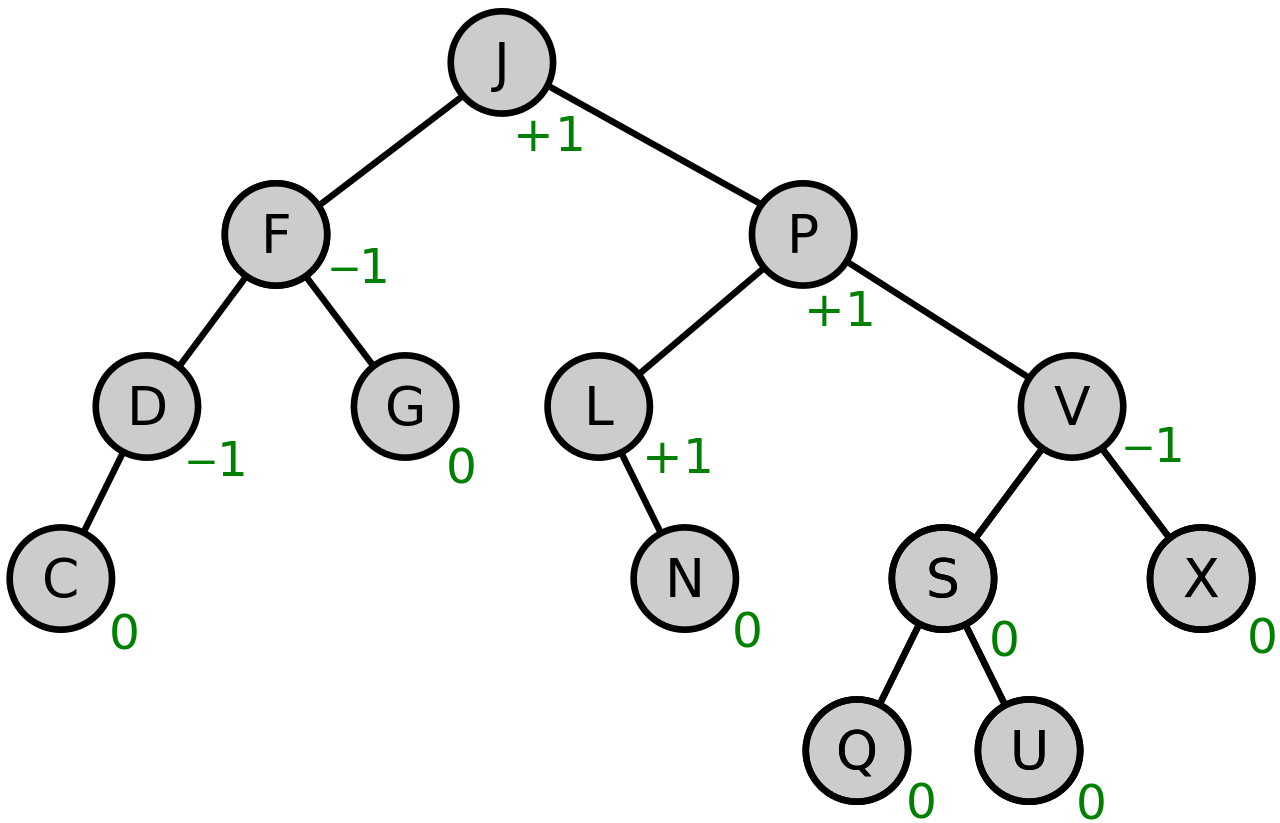
\includegraphics[width=0.5\textwidth]{AVL_tree.png}
    \caption*{Ejemplo de un árbol AVL, con el factor de balanceo de cada nodo.}
\end{figure}

\subsubsection{Cota sobre altura}

Para demostrar que, para todo AVL $T$ de $n$ nodos, $H(T) <= \log_k{n}$, demostramos que $k^{H(T)} <= n$. Si consideramos los AVLs con una altura $h$ de mínima cantidad de nodos, llamados árboles de Fibonacci de orden $h$, se tiene que sus subárboles también son árboles de Fibonacci, porque deben ser AVLs (por propiedad de AVL) y de cantidad de nodos mínima (en otro caso, el árbol no sería mínimo). Además, uno debe ser de orden $h - 1$ y el otro de $h - 2$, debido a que todos los árboles de altura $h$ tienen algún subárbol (derecho o izquierdo) de altura $h - 1$, y en este caso el otro puede tener a lo sumo $1$ unidad de diferencia (podría ser de la misma altura, pero en ese caso habría árboles con menos nodos). Esto implica que, si $AF_h$ es un árbol Fibonacci de orden $h$:
$$|AF_{h+2}| = |AF_{h+1}| + |AF_h| + 1$$

Esta recurrencia es muy similar a la definición de la secuencia de Fibonacci, $F_{i+2} = F_{i+1} + F_i$. De hecho:
$$|AF_i| = F_{i+2} - 1$$

Como la secuencia de Fibonacci crece exponencialmente (lo cual implica que $|AF_h| \in \BigOmega{k^h}$ para algún $k$) y, por definción, $|T| > |AF_h|$ para todo árbol AVL $T$ de altura $h$, la cantidad de nodos de cualquier árbol crece exponencialmente con respecto a su altura, lo cual implica que la altura crece logarítmicamente con respecto a la cantidad de nodos ($H(T) \in \log{n}$).

\subsubsection{Algoritmos}

La estructura AVL mantiene el $FDB$ de cada nodo interno, para facilitar las operaciones de rebalanceo.

\begin{itemize}
    \item \textbf{Inserción}: La inserción de un AVL consta de 2 pasos. Primero se debe insertar el nodo de la misma forma que para un ABB, y luego realizar \textit{rotaciones} en caso de que el árbol haya quedado demasiado (es decir, queda con un factor de balanceo de $\pm 2$). Las rotaciones son operaciones que preservan la propiedad de ABB, y se realizan de la siguiente manera:
          \begin{figure}[H]
              \centering
              \includegraphics*[width=0.5\textwidth]{AVL_rotation.png}
              \caption*{Ilustración de una rotación y su inversa}
          \end{figure}

          Las rotaciones aplicadas se dividen en cuatro casos, donde se toma como referencia el nodo desbalanceado:
          \begin{itemize}
              \item \textbf{RR}: Inserción en el subárbol derecho de un hijo derecho.
              \item \textbf{LR}: Inserción en el subárbol izquierdo de un hijo derecho.
              \item \textbf{RL}: Inserción en el subárbol derecho de un hijo izquierdo.
              \item \textbf{LL}: Inserción en el subárbol izquierdo de un hijo izquierdo.
          \end{itemize}

          Los casos LL y RR se pueden resolver con una única rotación: se rota a la derecha/izquierda el hijo del nodo desbalanceado. Por otro lado, los casos LR y RL requieren 2 rotaciones: una para el hijo, de forma que quede el caso RR o LL, y otra en el sentido contrario.

          La complejidad de este algoritmo está dada por la complejidad de sus pasos:
          \begin{enumerate}
              \item Buscar la posición apropiada del nodo a insertar -- $\BigTheta{\log{n}}$.
              \item Recalcular los $FDB$ -- $\BigTheta{\log{n}}$.
              \item Aplicar la/s rotación/es correspondiente/s -- $\BigTheta{1}$.
          \end{enumerate}

    \item \textbf{Borrar}: La operación de borrado se puede definir facilmente en términos de las anteriores:
          \begin{enumerate}
              \item Borrar el nodo como en un ABB tradicional.
              \item Recalcular los $FDB$ en la rama en que ocurrió el borrado (a lo sumo son $\log{n}$ nodos).
              \item \underline{Para cada nodo} con factor de balanceo $\pm 2$, hacer una rotación simple o doble (a lo sumo $\log{n}$ rotaciones).
          \end{enumerate}


\end{itemize}

Las operaciones de inserción, búsqueda y borrado terminan siendo de complejidad $\BigTheta{\log{n}}$ gracias a la cota que asegura el balanceo en altura de los AVLs.

\section{Tries}

La motivación para esta estructura de datos es obtener una implementación de los conjuntos/diccionarios con operaciones menos dependientes de la cantidad de claves, mantiniendo un rendimiento razonable en función del tamaño. Los \textit{tries} se basan en comparar partes claves parciales, en lugar de completas, lo cual las hace ideales para situaciones donde se usan strings como tipo de clave. La desventaja es que algunas implementaciones pueden requerir mucha memoria.

\subsection{Árboles de búsqueda digital}

Los \textit{árboles de búsqueda digital} (ABD) son similares a los ABB, en el sentido que para buscar una clave, se realiza una serie de comparaciones a lo largo del árbol. Sin embargo, algunas de estas comparaciones no son entre claves en sí, sino sus símbolos (bits, dígitos, caracteres, etc.), y son estas las que determinan las posiciones de las claves. La regla es que cada nodo se encuentra en una posición determinada por un prefijo de cierta longitud, y sus hijos son aquellas claves que comparten ese prefijo.

La inserción de una nueva clave se logra de la siguiente manera: se recorre el árbol utilizando los símbolos de la clave, hasta llegar a un nodo vacío, donde se coloca la clave. Por otro lado, la búsqueda recorre el árbol de la siguiente manera, comparando cada nodo con la clave buscada. Estas operaciones, dada una clave de $b$ símbolos, realizan $\log{n}$ comparaciones \underline{entre claves} en promedio\footnote{Siendo $n$ la cantidad de claves en el diccionario} y $b$ en el peor caso.

\subsection{Tries}

Un \textit{trie}, dado un alfabeto de $k$ elementos, es un árbol ${k+1}$-ario. En este caso, los ejes toman interés: representan los símbolos de las claves. Por lo tanto, cada subárbol representa al conjunto de claves que comienza con los símbolos de la rama entre la raíz y él. Los nodos internos no contienen claves: todas están en hojas, y se utiliza un símbolo especial para demarcar el fin de una clave (en este caso, $\$$).

    \label{fig-trie}
    \begin{figure}[H]
        \centering
        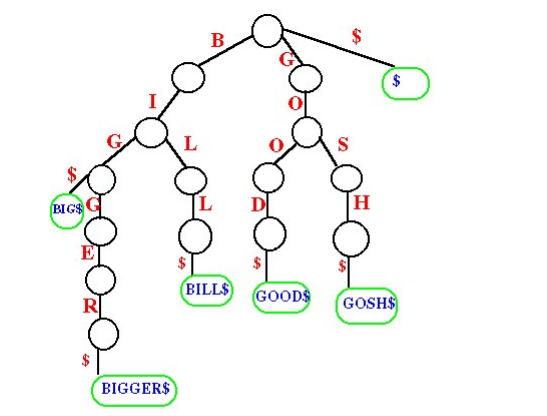
\includegraphics[width=0.5\textwidth]{trie.png}
        \caption*{Representación de un trie con claves BIG, BIGGER, BILL, GOOD, GOSH.}
    \end{figure}

    A diferencia de los ABD, la estructura resultante de un trie es independiente del orden en el que se agregan sus claves (es decir, hay un único trie para un conjunto de claves).

    La búsqueda/inserción de una clave $c$ se realiza siguiendo los ejes de la clave. Esto implica realizar a lo sumo $|c|$ comparaciones de símbolos. Suponiendo una distribución uniforme de las claves, las operaciones requieren $\BigO{\log{n}}$ comparaciones \underline{entre símbolos} en promedio y $|c|$ en el peor caso.

    \subsubsection{Comparación con AVL}

    Para comparar a los tries con los árboles AVL, se tiene que tener en cuenta el tamaño máximo de una clave, denotado $L$. En ambos casos las operaciones están acotadas por la altura de los árboles: para los tries esto es $L$, mientras que para un AVL esto es $\log{n}$. Por lo tanto, la eficiencia de los algoritmos dependerá de la relación entre estos dos valores.

    \subsubsection{Representación}

    Las dos posibles representaciones de un trie se corresponden en las dos maneras de representar secuencias: memoria estática (arreglos) y memoria dinámica (listas). Esto se debe a que se está representando un árbol ${k+1}$-ario, y por lo tanto cada nodo debe guardar una referencia a todos sus hijos.

    \begin{itemize}
        \item \underline{Arreglos}: Cada nodo interno cuenta con un arreglo de punteros a sus subárboles, donde las posiciones de ese arreglo representan las aristas de los símbolos. Transitar el árbol se vuelve simple: solo hace falta acceder a las posiciones correspondientes de los arreglos para cada símbolo de la clave buscada/insertada. Sin embargo, esta implementación puede ser extremadamente ineficiente en términos de memoria, en especial cuando el alfabeto es grande y la cantidad de claves chica. Esto se podría mitigar agrupando los caracteres poco frecuentes.
        \item \underline{Listas}: Los hijos de cada nodo se encuentran en una lista enlazada (opcionalmente ordenada), lo cual hace que recorrer el árbol requiera recorrer cada una de las listas de una rama de nodos. Esto es solo es eficiente en términos de tiempo cuando hay pocas claves, pero es mucho más eficiente en términos de espacio que la opción anterior.
    \end{itemize}

    \subsubsection{Tries compactos}

    Los \textit{tries compactos} son similares a los tries, pero compactan las cadenas que llevan hacia las hojas. Esto significa que, para cada clave, solo hay nodos internos para el prefijo más largo que comparte con alguna otra clave.

    \begin{figure}[H]
        \centering
        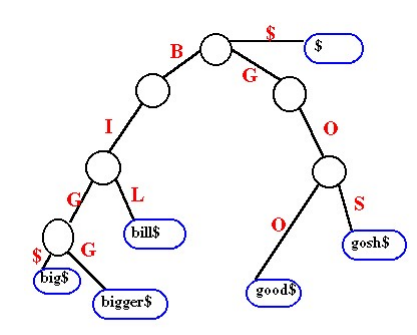
\includegraphics[width=0.5\textwidth]{trie_compacto.png}
        \caption*{Representación de un trie compacto equivalente al de la \hyperref[fig-trie]{figura anterior}.}
    \end{figure}

    \subsubsection{Tries PATRICIA}

    Los \textit{tries PATRICIA} (Practical Algorithm To Retrieve Information Coded In
    Alphanumeric) son una versión más compacta aún de los tries compactos. En este caso, solo hay nodos en las posiciones donde 2 o más claves difieren, así que se minimiza la cantidad de nodos internos.

    \begin{figure}[H]
        \centering
        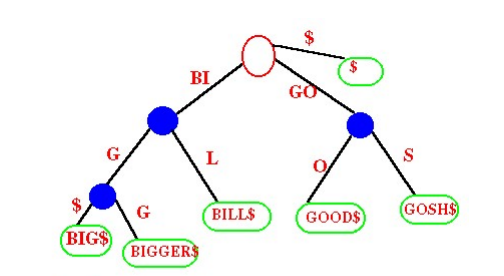
\includegraphics[width=0.5\textwidth]{trie_patricia.png}
        \caption*{Representación de un trie PATRICIA equivalente al de la \hyperref[fig-trie]{figura anterior}.}
    \end{figure}

    La altura de un árbol PATRICIA está acotada por el número de claves además de la cota anterior (la longitud de la clave más larga).

    \section{Tablas de hash}
    \label{sec-hash-tables}

    Las \textit{tablas de hash} son una implementación de conjunto/diccionario utilizada extensamente en la computación moderna. Resultan particularmente útiles en aplicaciones con acceso a memoria secundaria, donde representan el costo predominante en tiempo.

    Son una especie de generalización del concepto de arreglo, donde se pueden utilizar índices distintos de los números entre $0$ y $n-1$ (como strings).

    \subsection{Hashing}

    Para lograr indexar la estructura utilizando otros tipos de datos, se aplica una función de correspondencia entre el tipo y un entero. Esta transformación depende de la implementación, pero \underline{debe} ser una función ($x = y \implies f(x) = f(y)$), y es ideal que sea inyectiva ($x = y \impliedby f(x) = f(y)$).

    Esta función se denomina \textit{hash}, y tiene la forma $h: K \rightarrow \{0, ..., n-1\}$ donde $K$ es el génergo que contiene a las posibles claves del diccionario y n es el tamaño de la tabla de hash.

    \subsection{Colisiones}

    Una función de hash perfecta sería inyectiva, lo cual implicaría que $|K| \leq n$ (la tabla de hash es al menos tan grande como el conjunto de claves posibles). Esto no resulta factible en la práctica, así que toda tabla de hash tiene que tener una forma de manejar \textit{colisiones} entre distintas claves con el mismo hash. Estos métodos se denominan \textit{resolución de colisiones}.

    Más allá de la resolución de colisiones, una buena función de hash debería cumplir la propiedad de \textit{uniformidad simple}, que implica que todos los elementos de su imagen tienen probabilidades similares de ser resultado de alguna clave. Formalmente:
$$\forall i \in \{0, ..., n-1\},\ \sum_{k \in K \mid h(k) = i} P(k) \approx \frac{1}{n}$$

Debido a la dificultad (o imposibilidad) estimar la distribución de las claves, esta propiedad no suele cumplirse en la práctica, así que se intenta encontrar una función independiente de la distribución.

\subsubsection{Direccionamiento por concatenación}

El \textit{direccionamiento cerrado} o \textit{direccionamiento por concatenación} es simple: a cada posición $i$ del arreglo se le asigna una lista que contiene las claves $k$ (y significados asociados) tales que $h(k) = i$. La búsqueda e inserción de una clave $k$ requiere recorrer la lista asociada a $h(k)$ para encontrarla (o verificar que no está), así que su complejidad es proporcional a la longitud de dicha lista. Si definimos el \textit{factor de carga} $\alpha = \frac{n}{|T|}$, donde $n$ es la cantidad de llaves en la tabla $T$ y $|T|$ su tamaño máximo, se puede demostrar lo siguiente\footnote{Asumiendo la hipótesis de simplicidad uniforme de $h$}:
\begin{itemize}
    \item Una búsqueda fallida requiere en promedio tiempo $\BigTheta{1 + \alpha}$.
    \item Una búsqueda exitosa requiere en promedio tiempo $\BigTheta{1 + \frac{\alpha}{2}}$.
\end{itemize}

Por ende, esta implementación tiene operaciones de complejidad $\BigO{1}$ en promedio, siempre que $n$ sea cercano a $|T|$.

\subsubsection{Direccionamiento abierto}

En los métodos de \textit{direccionamiento abierto}, todos los elementos se almacenan directamente en la carga, y las colisiones se resuelven dentro de la misma. En este caso, redefinimos la función de hashing a $h(k, i)$, que representa la dirección del $i$-ésimo intento de guardado. Cuando se intenta insertar una clave en una posición ocupada, se sigue intentando hasta encontrar una posición libre. Un esquema del algoritmo de inserción sería:
\begin{algorithm}[H]
    \caption*{Insertar en tabla de hash con direccionamiento abierto}
    \begin{algorithmic}
        \Function{insertar}{\textbf{significado} $s$, \textbf{clave} $k$, \textbf{diccionario} $T$}
        \State $i \gets 0$
        \While{\textsc{ocupado?}($T[h(k, i)]$) $\land\ i < |T|$}
        \State $i \gets i + 1$
        \EndWhile
        \If{$i < |T|$}
        \State $T[h(k, i)] \gets (k, s)$
        \Else
        \State \textbf{OVERFLOW}
        \EndIf
        \EndFunction
    \end{algorithmic}
\end{algorithm}

La búsqueda se realiza análogamente, realizando intentos sucesivos hasta que se encuentra la clave, o se llega a una posición vacía (que implica que la clave nunca fue agregada).
\begin{algorithm}[H]
    \caption*{Buscar en tabla de hash con direccionamiento abierto}
    \begin{algorithmic}
        \Function{buscar}{\textbf{clave} $k$, \textbf{diccionario} $T$}
        \State $i \gets 0$
        \While{\textsc{ocupado?}($T[h(k, i)]$) $\land\ T[h(k, i)] \neq \perp \ \land\ i < |T|$}
        \State $i \gets i + 1$
        \EndWhile
        \If{$i < |T| \land T[h(k, i)] \neq \perp$}
        \State \Return T[h(k, i)]
        \Else
        \State \Return $\perp$
        \EndIf
        \EndFunction
    \end{algorithmic}
\end{algorithm}

Esto presenta un problema: si se inserta una clave, luego se insertan otras que colisionan con ella, y se elimina la primera, las otras claves quedarían inaccesibles (porque el algoritmo retornaría falso al encontrar $\perp$ en el primer intento). Esto se puede solucionar cambiando el método de borrado: en vez de usar $\perp$, se puede usar un valor especial que indica que fue borrado.

La forma en la que se relaciona $h(k, i)$ con $h(k, i + 1)$ se denomina \textit{método de barrido}, y algunos son:
\begin{itemize}
    \item \textbf{Barrido linear}: $h(k, i + 1)$ = $h(k, i) + 1$\footnote{En todos los casos la función $h$ trabaja con aritmética$\mod{|T|}$, para evitar salir del rango del arreglo} (o, equivalentemente, $h(k, i)$ = $h(k) + i$). Es simple, pero es propensa a la \underline{aglomeración primaria}: si dos secuencias de barrido tienen una colisión, siguen colisionando, y se producen largos tramos de aglomeración ($h(k_1, i) = h(k_2, j) \implies h(k_1, i + a) = h(k_2, j + a) \forall a \in \mathbb{N}$).
    \item \textbf{Barrido cuadrático}: En este caso, $h(k, i) = h(k) + c_1 i + c_2 i^2$, con $c_1, c_2$ constantes. Esto evita el problema anterior, pero sufre de \underline{aglomeración secundaria}, donde si dos claves colisionan en el primer intento, colisionan siempre.
    \item \textbf{Hashing doble}: Se define $h(k, i) = h_1(k) + i h_2(k)$, donde $h_1, h_2$ son dos funciones de hashing distintas. Esto reduce la aglomeración secundaria (y no tiene aglomeración primaria). El problema con este esquema es que es ineficiente en su uso del caché de la CPU (debido a que las claves colisionadas podrían quedar en posiciones distantes).
\end{itemize}

\subsection{Funciones de hash}

\subsubsection{Prehashing}

El \textit{prehashing} es la etapa del hashing en la que se pasa del tipo utilizado como clave a un entero. El método debe definirse para cada tipo deseado y, como siempre, es deseable que la función tenga pocas colisiones (o sea inyectiva).

\subsubsection{Métodos de hash}

Una vez que se tiene un número, existen distintos métodos de hashing:
\begin{itemize}
    \item \textbf{División}: $h(k) = k\mod{|T|}$. Este método es simple de implementar y rápido de calcular. Para evitar colisiones, es ideal que el tamaño de la tabla sea un número primo no muy cercano a una potencia de $2$.
    \item \textbf{Partición}: Se particiona la clave $k$ en $k_1, k_2, ..., k_n$, y luego se define $h(k) = f(k_1, k_2, ..., k_n)$ para alguna función $f$. La idea es romper los patrones que tenían los datos para lograr una distribución uniforme.
    \item \textbf{Extracción}: Se usa una sola parte de la clave para calcular el hash, la que más varíe dentro del conjunto.
\end{itemize}

\section{Colas de prioridad}

El tipo abstracto \textit{cola de prioridad} es similar a una cola o pila donde, en lugar de decidir el siguiente elemento a desencolar a través del orden de inserción, se utiliza una relación de prioridad $<_{\alpha}$. Esto se puede representar utilizando un \hyperref[subsec-avl]{AVL}, donde la búsqueda y el desencolado se pueden implementar en tiempo logarítmico. En esta sección, exploraremos una implementación más elegante y sencilla (y que posibilita algunas operaciones adicionales).

\subsection{Heap}

Un \textit{heap} es un árbol binario perfectamente balanceado que cumple el siguiente invariante: la prioridad de cada nodo es mayor/menor a la de sus hijos. Esto implica que todo subárbol del heap es un heap. Opcionalmente (y siempre en nuestro caso) puede ser \textit{izquierdista}, donde el último nivel se llena de izquierda a derecha. Cuando las prioridades son mayores a las de los hijos, se tiene un máx-heap, mientras que cuando son menores se tiene un mín-heap.

\subsubsection{Representaciones}

El heap admite cualquier representación de árboles binarios. Una opción podría ser la tradicional, donde cada nodo contiene su valor junto con punteros a sus hijos, pero en este caso la representación con arrays es particularmente eficiente. Consiste en almacenar los valores de los nodos un array, y relacionar a los padres con sus hijos a través de las posiciones: si $v$ es un nodo almacenado en la posición $p(v)$, su hijo izquierdo se almacena en $2p(v) + 1$, y el derecho en $2p(v) + 2$.

Los arrays tienen la ventaja de ser muy eficientes en términos de espacio y de utilización de caché de CPU, pero su tamaño estático hace necesaria el uso de técnicas adicionales para agregar elementos (como la implementada en los arreglos dimensionables).

\subsubsection{Algoritmos}

\begin{itemize}
    \item \textbf{Próximo}: El elemento de prioridad máxima siempre se encuentra en la posición $0$ del arreglo, y la complejidad de acceder a él es siempre $\BigTheta{1}$.
    \item \textbf{Encolar}: El algoritmo de inserción consiste en insertar el elemento en la siguiente posición vacía (dada por el orden izquierdista) y \textit{percolar} hacia arriba hasta que se restaure el invariante de heap. Esto implica intercambiar a un nodo con su padre en caso de que este tenga prioridad mayor.
          \begin{algorithm}[H]
              \caption*{Insertar en heap}
              \begin{algorithmic}
                  \Function{Insertar}{\textbf{elemento} $e$, \textbf{heap} $H$}
                  \State Insertar $e$ en la última posición de $H$.
                  \While{$e \text{ no está en la raíz} \land_L e > \textsc{Padre}(e, H)$}
                  \State Intercambiar $e$ con \textsc{Padre}($e$, $H$).
                  \EndWhile
                  \EndFunction
              \end{algorithmic}
          \end{algorithm}

          Este algoritmo corre en tiempo proporcional a la altura del árbol que, por ser perfectamente balanceado, está acotada por $\log_2{n}$ (y por ende se tiene una complejidad de $\BigTheta{\log{n}}$).
    \item \textbf{Desencolar}: El algoritmo de desencolado es parecido al de inserción: se intercambia el elemento de la raíz con el último, eliminarlo, y percolar hacia abajo la nueva raíz este hasta restaurar el invariante de heap.
          \begin{algorithm}[H]
              \caption*{Desencolar en heap}
              \begin{algorithmic}
                  \Function{Desencolar}{\textbf{heap} $H$}
                  \State $result \gets\textsc{Raíz}(H)$
                  \State Intercambiar \textsc{Raíz}($H$) con su último elemento.
                  \State Eliminar el último elemento.
                  \State $e \gets \textsc{Raíz}(H)$
                  \While{$e \text{ tiene algún hijo} \land_L e < \max{\{\textsc{HijoIzq}(e), \textsc{HijoDer}(e)\}}$}
                  \State Intercambiar $e$ con $\max{\{\textsc{HijoIzq}(e), \textsc{HijoDer}(e)\}}$.
                  \EndWhile
                  \State \Return $result$
                  \EndFunction
              \end{algorithmic}
          \end{algorithm}

          Al igual que en el algoritmo de inserción, el de desencolamiento tiene complejidad $\BigTheta{\log{n}}$.
\end{itemize}

\subsubsection{Array a Heap}
\label{subsubsec-floyd}

La operación de transformar un array a un heap se puede implementar simplemente: basta con encolar uno por uno cada elemento del array. De esta forma se logra una complejidad temporal de $\BigTheta{n\log{n}}$. Esto se puede mejorar a través del algoritmo de Floyd, que está basado en \textit{heapificar} los subárboles del árbol representado por el arreglo, empezando desde el anteúltimo nivel hacia arriba. Esto se logra a través de la operación \textsc{Bajar}, que es equivalente a la de percolar hacia abajo en el algoritmo de desencolado. Si se aplica \textsc{Bajar} a todos los elementos del arreglo de atrás para adelante, se consigue un heap, y la complejidad es de $\BigTheta{n}$.

\section{Ordenamiento}

Ahora detallamos varios métodos de ordenamiento de secuencias.

\subsection{Selection Sort}

\textit{Selection sort} es un algoritmo simple, que se basa en tomar para cada posición el mínimo del subarreglo desordenado. El ciclo exterior se caracteriza por el siguiente invariante para cada iteración $i$:
\begin{enumerate}
    \item Los elementos de $arr[0...i]$ son los $i+1$ más pequeños de todo el arreglo (y menores a todos los demás).
    \item Los elementos de $arr[0...i]$ están ordenados.
    \item $arr$ es una permutación del arreglo original lo cual, junto con 1., implica que $arr[i+1...n)$ contiene a los $n - i - 1$ elementos más grandes del arreglo original).
\end{enumerate}

\begin{algorithm}[H]
    \caption*{Selection Sort}
    \begin{algorithmic}
        \For{$i \in \{0, ..., n-2\}$}
        \State $m \gets \text{arg} \min{arr[i, n)}$
        \State \textsc{Swap}($arr$, $i$, $m$)
        \EndFor
    \end{algorithmic}
\end{algorithm}

Como encontrar la posición del elemento mínimo de un arreglo es $\BigTheta{n}$ (y swappear es constante), este algoritmo tiene complejidad $\sum_{i=1}^{n-1} \BigTheta{i} = \BigTheta{\frac{n(n-1)}{2}} = \BigTheta{n^2}$. El algoritmo realiza la misma cantidad de operaciones para todos los arreglos, así que este es el costo peor, promedio y mejor.

\subsection{Insertion Sort}

Al igual que selection sort, \textit{insertion sort} mantiene un subarreglo ordenado, solo que en este caso este es una permutación del subarreglo correspondiente original. Su invariante es el siguiente:
\begin{enumerate}
    \item Los elementos de $arr[0, i]$ son una permutación de los del arreglo original.
    \item Los elementos de $arr[0, i]$ están ordenados.
    \item El arreglo $arr$ es una permutación del arreglo original.
\end{enumerate}

\begin{algorithm}[H]
    \caption*{Insertion Sort}
    \begin{algorithmic}
        \For{$i \in \{0, ..., n-2\}$}
        \While{$i > 0 \land_L arr[i] < arr[i - 1]$}
        \State \textsc{Swap}($arr$, $i$, $i-1$)
        \State $i \gets i - 1$
        \EndWhile
        \EndFor
    \end{algorithmic}
\end{algorithm}

Análogamente al caso de selection sort, al realizar a lo sumo $i$ comparaciones en cada iteración, el algoritmo tiene complejidad de peor caso $\BigTheta{n^2}$. Sin embargo, el ciclo interno puede terminar antes, y el algoritmo puede hacer $\BigTheta{n}$ operaciones en el mejor caso (cuando el arreglo ya se encuentra ordenado).

Este algoritmo es el primero que analizamos que tiene la propiedad de ser \textit{estable}: se mantiene el orden previo de elementos con igual clave. Esto es útil a la hora de realizar varios ordenamientos con distintas claves, ya que se preserva cualquier orden previo que podía existir. En realidad, selection sort puede volverse estable con una modificación: en vez de swappear el elemento mínimo con la posición actual, se lo inserta, corriendo los elementos posteriores.

\subsection{Heap Sort}

El algoritmo \textit{heap sort} se basa en aprovechar la estructura de heap. Podría pensarse como una versión del selection sort, donde primero se heapifica el arreglo (a través del \hyperref[subsubsec-floyd]{algoritmo de Floyd}) y luego se obtiene el elemento mínimo en cada iteración desencolando en el heap. Esto se puede realizar en tiempo $\BigTheta{n\log{n}}$ (son $n$ desencolados).

El heap sort puede implementarse de forma \textit{in-place}, es decir, usando una cantidad constante de memoria adicional. Para ello, se debe convertir el arreglo original en un máx-heap, e ir colocando los elementos desencolados al final del arreglo. De esta manera, las operaciones de heap se realizan sobre el subarreglo desordenado, y luego de $n$ iteraciones el array queda ordenado de menor a mayor. Sin embargo, este algoritmo no es estable.

\subsection{Merge Sort}

El algoritmo \textit{merge sort} es un ejemplo de la metodología \hyperref[sec-dyc]{``Divide \& Conquer``}, y sigue el siguiente esquema recursivo:
\begin{itemize}
    \item \textbf{Si $n < 2$}: Es el caso base, y el arreglo está ordenado (tiene $1$ o $0$ elementos).
    \item \textbf{Si no}:
          \begin{enumerate}
              \item Dividir el arreglo en dos mitades de igual tamaño.
              \item Aplicar merge sort en cada mitad.
              \item \textit{Mergear} las mitades ordenadas (se puede implementar en tiempo lineal).
          \end{enumerate}
\end{itemize}

El costo de este algoritmo está dado por la recurrencia $T(n) = 2 T(\frac{n}{2}) + \BigTheta{n}$, con el caso base $T(1) = \BigTheta{1}$. Esto está acotado por $\BigTheta{n\log{n}}$.

\subsection{Quick Sort}

El \textit{quick sort} es otro algoritmo Divide \& Conquer. A diferencia de merge sort, la división en cada paso no se realiza a la mitad, sino que se elige un \textit{pivot}, y se particiona el arreglo entre menores y mayores a ese elemento. Luego, el esquema sería el siguiente:
\begin{itemize}
    \item \textbf{Si $n < 2$}: Caso base, el arreglo está ordenado.
    \item \textbf{Si no}:
          \begin{enumerate}
              \item Se elije el pivot $p$.
              \item Se calculan las particiones $P_{< p}$ y $P_{\geq p}$.
              \item Se ordenan utilizando quick sort.
          \end{enumerate}

          Notar que en el último paso no hace falta mergear las particiones porque, al estar definidas en relación a $p$, basta con concatenarlas (los elementos mayores a $p$ son mayores que los menores a $p$ por transitividad).

\end{itemize}

La elección del pivot tiene un gran impacto en la complejidad temporal. Por ejemplo, si siempre se toma el primer elemento del arreglo como pivot, quicksort correrá en tiempo $\BigTheta{n^2}$ cuando la entrada ya está ordenada, ya que en cada paso de partición solo se reduce en $1$ el tamaño del subarreglo a ordenar (la ejecución sería equivalente a selection sort). Lo ideal sería tomar el elemento mediano, pero en la práctica es difícil encontrar ese elemento en tiempo lineal. En cambio, elegir un elemento al azar permite una complejidad promedio de $\BigTheta{n\log{n}}$.

La operación más compleja de este algoritmo es realizar la partición. Se puede implementar en tiempo lineal utilizando un algoritmo de $2$ punteros:

\begin{algorithm}[H]
    \caption*{Particionar un arreglo dada una posición de pivot}
    \begin{algorithmic}
        \Function{Particionar}{\textbf{arreglo} $arr$, \textbf{posición} $p$}
        \State $pivot \gets arr[p]$
        \State \textsc{Swap}($arr$, $p$, $0$)
        \State \textsc{Swap}($arr$, arg $\max{arr}$, $|arr| - 1$)
        \State $lower \gets 1, upper \gets |arr| - 2$
        \While{$lower \leq upper$}
        \While{$arr[lower] < pivot$}
        \State $lower \gets lower + 1$
        \EndWhile
        \While{$arr[upper] \geq pivot$}
        \State $upper \gets upper - 1$
        \EndWhile
        \If{$lower \leq upper$}
        \State \textsc{Swap}($arr$, $lower$, $upper$)
        \EndIf
        \EndWhile
        \EndFunction
    \end{algorithmic}
\end{algorithm}

\subsection{Optimalidad}

Para el problema de ordenamiento, se puede demostrar un \textit{lower bound} de $\BigOmega{n\log{n}}$, es decir, la complejidad mínima que tiene que cumplir un algoritmo que lo resuelve. En realidad, la cota vale para algoritmos que están basados en comparaciones: si se cuenta con alguna hipótesis adicional (como elementos acotados por un rango), se pueden implementar algoritmos más rápidos (como counting sort).

Para demostrar eso, vamos a asumir que todas as comparaciones tienen la forma de $a_i$ < $a_j$, y que el resultado es siempre $verdadero$ o $falso$. Utilizamos la herramienta de \textit{árboles de decisión}, cuyas ramas representan todos los posibles caminos de cómputo que podría tomar un algoritmo. Los nodos internos representan las distintas comparaciones que se realizan, mientras que cada hoja se corresponde con una posible output del algoritmo. La altura del árbol representa la cantidad máxima de ejecuciones posibles.

En el caso del ordenamiento, hay una hoja por cada permutación posible, así que tiene $n!$ nodos hoja. Esto implica que la altura mínima es $\BigOmega{\log{n!}} = \BigOmega{n\log{n}}$. Por ende, los algoritmos como merge sort y heap sort tiene una complejidad asintóticamente óptima.

\section{Dividir y Conquistar}
\label{sec-dyc}

\subsection{Definción}

\textit{Dividir y Conquistar} (DyC) es una técnica de diseño de algoritmos con el siguiente esquema general:
\begin{enumerate}
    \item \textbf{Divide}: Dividir el problema en \textit{subproblemas} más chicos, resolviéndolos recursivamente.
    \item \textbf{Conquer}: Combinar las soluciones de los subproblemas para obtener la solución del problema original.
\end{enumerate}

Esta metodología tiene sentido siempre y cuando la división y combinación sean implementables de forma eficiente.
\begin{algorithm}[H]
    \caption*{Esquema general de DyC}
    \begin{algorithmic}
        \Function{DyC}{\textbf{instancia} $X$}
        \If{$X$ es suficientemente chico} \Comment{Caso Base}
            \State \Return \textsc{AdHoc}($X$) 
        \Else \Comment{Caso Recursivo}
            \State $X_1, X_2, ..., X_k \gets \textsc{Descomponer}(X)$
            \For{$i \in \{1, 2, ..., k\}$}
            \State $Y_i \gets DC(X_i)$
            \EndFor
            \State \Return \textsc{Combinar}($Y_1, Y_2, ..., Y_k$)
        \EndIf
        \EndFunction
    \end{algorithmic}
\end{algorithm}

\subsection{Análisis de complejidad}

En un algoritmo típico de DyC, se divide el problema en $a$ subproblemas de tamaño $\frac{n}{c}$, y el costo de la división en sí junto con la combinación está dado por una función $f(n)$. Si $f(n) = bn^d$, entonces se tiene:
\begin{align*}
    T(n) & = aT\left(\frac{n}{c}\right) + bn^d \\
    T(n) & = bn^d \left(\sum_{i=0}^{\log_c{n}} \left(\frac{a}{c^d}\right)^i\right)
\end{align*}

Esta recurrencia puede ser resuelta a través de un análisis de casos:
\begin{itemize}
    \item Cuando $a = 1, d = 0$ (un solo subproblema y combinación de costo constante, como en la búsqueda binaria):
        $$T(n) \in \BigO{\log{n}}$$
    \item Cuando $d = 1$ y:
     \begin{itemize}
        \item $a < c$ (``pocos subproblemas''):
            $$T(n) \in \BigO{n}$$
        \item $a = c$ (``conquer lineal'', como en merge sort):
            $$T(n) \in \BigO{n\log{n}}$$
        \item $a > c$ (``muchos subproblemas''):
            $$T(n) \in \BigO{n^{\log_c{a}}}$$
     \end{itemize}
\end{itemize}

Para otros costos de conquer $f(n)$, se puede aplicar el \textbf{Teorema Maestro}:

\begin{theorem*}
    Si se tiene una relación de recurrencia de la siguiente forma:
    $$
    T(n) =
    \begin{cases}
        a T\left(\frac{n}{c}\right) + f(n) & \text{si } n > 1 \\
        1                       & \text{si } n = 1
    \end{cases}
    $$

    Su fórmula cerrada es:
    \begin{enumerate}
        \item Cuando $f(n) \in \BigO{n^{\log_c{a} - \epsilon}}$ para algún $\epsilon > 0$.
            $$T(n) \in \BigTheta{n^{\log_c{a}}}$$
        \item Cuando $f(n) \in \BigTheta{n^{\log_c{a}}}$
            $$T(n) \in \BigTheta{n^{\log_c{a}} \log{n}}$$
        \item Cuando $f(n) \in \BigOmega{n^{\log_c{a} + \epsilon}}$ y $a f\left(\frac{n}{c}\right) < k k(n)$ para $k < 1$ y $n$ suficientemente grande.
            $$T(n) \in \BigTheta{f(n)}$$
    \end{enumerate}

    En los casos 1. y 3., se cumple $T(n) \in \BigTheta{f(n) + n^{\log_c{a}}}$.
\end{theorem*}

\section{Algoritmos en memoria secundaria}

En esta sección vamos a considerar algoritmos para realizar búsqueda y ordenamiento en ambientes donde se cuenta con mucho espacio de almacenamiento, pero el acceso a ese espacio es lento. En particular, para el caso de discos duros, el tiempo de acceso está dominado por la operación de encontrar el dato a leer (el ``posicionamiento'' del cabezal), así que acceder a un byte tiene un costo similar a acceder a un bloque contiguo.

Si se cuenta con un método con buena \textit{localidad de referencia}, se puede implementar directamente y delegar el acceso a memoria al mecanismo de \textit{memoria virtual} del sistema operativo.

\subsection{Ordenamiento--fusión}

Una estrategia para ordenar un archivo presente en una memoria de acceso secuencial es seguir el siguiente esquema:
\begin{itemize}
    \item Dividir el archivo en bloques que entren en memoria.
    \item Ordenar esos bloques.
    \item Fusionarlos/Mergearlos.
\end{itemize}

Vemos 3 ejemplos de algoritmos de ordenamiento-fusión. Su complejidad se mide en \textit{pasadas} por memoria externa, porque ese es el costo que predomina debido al tiempo de búsqueda mencionado.

\subsubsection{Fusión múltiple equilibrada}

Para el algoritmo de \textit{fusión múltiple equilibrada}, se supone que se tiene que ordenar un archivo de registros presente en una cinta, que sólo puede ser accedido secuencialmente. También se dispone de una memoria con espacio para un número constante de registros (denotado $m$), y una cantidad arbitraria de cintas auxiliares. El procedimiento es el siguiente:
\begin{enumerate}
    \item En la primera pasada se realiza el siguiente ciclo: Mientras que queden elementos en la cinta, leer bloques de $m$ elementos, ordenarlos, y escribirlos en la cinta auxiliar $i$ para cada $i \in \{1, ..., p\}$.
    \item En la segunda pasada se realiza este otro ciclo: Mientras haya bloques de $p$ en las $p$ cintas auxiliares, fusionarlos a $p$ vías, armando bloques de $p^2$ en nuevas cintas auxiliares.
    \item El paso 2. se repite hasta que todos los bloques queden en una sola cinta, que representan al la secuencia ordenada.
\end{enumerate}

Este algoritmo realiza $\log_p{\frac{n}{m}}$ pasadas cuando se ordenan $n$ registros con memoria interna de tamaño $m$ y fusiones a $p$ vías.

\subsubsection{Selección por sustitución}

El algoritmo de \textit{selección por sustitución} es una versión modificada de la fusión múltiple equilibrada. La idea principal es utilizar una cola de prioridad de tamaño $m$ para armar los bloques iniciales, ``pasando'' los elementos a través de ella al desencolar el menor y sustituirlo por el siguiente. Pero, si el elemento nuevo es menor al que acaba de salir, se lo marca como si fuera mayor, hasta que alguno de los nuevos elementos llegue al primer lugar de la cola, en cuyo caso se inicia un nuevo bloque (que se escribe en otra cinta).

Esta modificación permite construir bloques más largos que los de $m$ registros de la fusión múltiple equilibrada original: para secuencias aleatorias, las secuencias armadas son de largo promedio $2m$. Esto permite reducir la cantidad de pasadas en $1$.

\subsubsection{Fusión Polifásica}

La \textit{fusión polifásica} es otra versión de la fusión múltiple equilibrada, que se enfoca en reducir la cantidad de cintas auxiliares necesarias. Si no se cuenta con las $p + 1$ necesarias para la fusión de $p$ vías, se puede hacer lo siguiente:
\begin{itemize}
    \item Distribuir los datos en todas las cintas menos una, aplicando la estrategia de ``fusión hasta el vaciado''.
    \item Cuando alguna de las cintas se vacía, rebobinarla y usarla como nueva cinta de salida
\end{itemize}

\subsection{Búsqueda externa}

La implementación de diccionarios en memoria externa es un problema común en aplicaciones como bases de datos o sistemas de archivos. Se toma el modelo de memoria de acceso a \textit{páginas}, bloques contiguos de datos.

\subsubsection{ISAM}

El método de \textit{acceso secuencial indexado} (ISAM) se basa en almacenar las claves del diccionario ordenadas en cada \textit{disco}\footnote{Disco es el antecesor de las página en la jerarquía de memoria, no necesariamente en disco duro en sí.} disponible, y además para todos construir un \textit{índice} que se almacena en la primera página de estos. Los índices indican, para cada página, cuál es la última clave de la página anterior. Para tamaños de página suficientemente grandes (donde no puede haber una página llena de un mismo índice), la búsqueda de una clave se puede realizar en $\log_2{\#discos}$ accesos a índices y un único acceso a la página . Esto se puede mejorar aún más a través de un \textit{índice maestro}, que indica qué claves están en cada disco y puede ser guardado en memoria principal.

Mantener los índices presenta un problema a la hora de insertar claves, por lo cual esto no suele usarse en la práctica.

\subsubsection{Árboles B}

Los \textit{Árboles B} son árboles completamente balanceados: todas las hojas están a la misma distancia de la raíz. No son binarios, es decir, cada nodo puede tener más de $2$ hijos. En el caso de la memoria secundaria, cada nivel se corresponde con un nivel en la jerarquía.

Un caso particular de los B-Trees son los \textit{Árboles 2-3-4}, donde cada nodo puede tener 2, 3 o 4 hijos. Por ejemplo, para los 3-nodos, la raíz contiene 2 valores ($c_1$ y $c_2$) y se cumple el siguiente invariante:
\begin{itemize}
    \item El hijo izquierdo contiene todas las claves menores a $c_1$.
    \item El hijo medio contiene todas las claves entre $c_1$ y $c_2$.
    \item El hijo derecho contiene todas las claves mayores a $c_2$.
\end{itemize} 

Para insertar un nuevo valor, se encuentra el nodo correspondiente. Si está saturado (es un 4-nodo), se \textit{parte} en 2 nodos y una de las claves se inserta en el nodo de arriba, partiéndolo si es necesario, y así sucesivamente. Otra posible solución es partir preventivamente todos los 4-nodos que se encuentren en el camino de descenso de la clave, asegurando que en la inserción final habrá lugar en el nodo padre.

Volviendo a los árboles B, la funcionalidad es igual a de los 2-3-4, pero cada nodo puede tener hasta $M$ hijos, y cuenta con un arreglo de $M-1$ claves. Para encontrar una clave, se debe realizar una búsqueda binaria para cada uno de los nodos. Luego, para utilizarlos en memoria secundaria, la idea es que cada nodo corresponda a una página de disco (incluyendo claves, significados y enlaces). En términos de complejidad, esta estructura puede realizar las operaciones de búsqueda, inserción y borrado en $\BigO{\log{n}}$ accesos de nodos, pero los algoritmos tienen cierta dificultad para implementarse.

\subsubsection{Hashing dinámico}

El \textit{hashing dinámico} o \textit{extensible} es un híbrido de los métodos anteriores: al igual que en los árboles B, los registros se almancenan en páginas que, al llenarse, se dividen en dos partes, mientras que también se mantiene un índice que se utiliza para encontrar la página que contiene los registros correspondientes a una clave, como en ISAM.

Este método requiere contar con una serie de funciones de hash distintas $h_1, h_2, ...$ que tienen como imagen el conjunto $\{0, 1\}$. Inicialmente, se cuenta con dos páginas, y cada registro se inserta según el valor de $h_1$. Cuando alguna página se llena, esta se parte en 2, donde los elementos se dividen según la siguiente función de hash. Siempre y cuando el árbol de índices entre en memoria, la búsqueda solo requiere un solo acceso a página y la inserción 3 (la página original y las 2 nuevas).

Para evitar borrar y crear páginas frecuentemente, la partición se puede realizar cuando una página llega a cierto umbral de su capacidad (por ejemplo, 80\%), así como la fusión de páginas (cuando ambas tengan un largo combinado de 20\% de una página). Otra consideración son las fusiones de hash: para mantener un árbol medianamente balanceado, es ideal que cada hash tenga buena uniformidad sobre las claves.

\section{Algoritmos probabilísticos}

\subsection{Definición}

Un algoritmo \textit{probabilístico} es uno que incorpora algún elemento de azar a su ejecución. Esto implica que no es determinístico: múltiples ejecuciones del algoritmo con la misma entrada pueden producir distintas salidas o tiempos de ejecución. En este caso, analizaremos algoritmos \textit{Las Vegas}, que son aquellos que siempre dan un resultado correcto, pero cuyo tiempo de ejecución es una variable aleatoria (un ejemplo sería quicksort con elección de pivot aleatorio). Los \textit{Montecarlo}, por otro lado, son aquellos que tienen alguna probabilidad de producir un resultado incorrecto.

\subsection{Skip lists}

Las \textit{skip lists} son una representación de diccionarios basada en listas enlazadas ordenadas. Una implementación directa tendría una complejidad de búsqueda de peor caso de $\BigO{n}$: la lista solo puede ser recorrida secuencialmente, y si el elemento se encuentra al final, hay que recorrerla toda. Esto puede ser acelerado ``salteando'' elementos, que se logra agregando referencias a nodos posteriores. Por ejemplo, si todos los nodos en posiciones pares tienen referencias a la siguiente posición par, la búsqueda se peude implementar en $\left\lceil \frac{n}{2} \right\rceil + 1$ lookups.

Las skip lists \textit{perfectas} extienden esta idea: cada $2^i$-ésimo nodo posee una referencia al nodo $2^i$ posiciones más adelante en la lista. Luego, la búsqueda de una clave $c$ se realiza análogamente a la búsqueda binaria: para cada nivel $i$, existen $2$ posibles rangos en los que podría encontrarse la clave, y se determina en cuál comparándola con el elemento en el medio. Por ende, se examinan a lo sumo $\log_2(n)$, y el número total de referencias es solo el doble de una lista enlazada tradicional.

Sin embargo, estas estructuras son demasiado rígidas, ya que es muy costoso mantener el invariante a la hora de insertar o borrar claves. Las skip lists normales \textit{randomizan} el requerimiento: al insertar un nodo, este es promocionado al nivel superior con una probabilidad de $\frac{1}{2}$ iterativamente (se frena cuando deja de ser promocionado o cuando llega al último nivel). Esto permite que la distribución de nodos en cada nivel sea equivalente a la de las skip lists perfectas, lo cual produce un costo de búsqueda promedio de $\BigO{log{n}}$.

\subsection{Splay trees}

Si se conocen de antemano las \textit{frecuencias de acceso} a cada clave de un diccionario, se puede construir un \textit{ABB óptimo}, donde la altura de cada elemento (que es proporcional a su tiempo de acceso) depende de su frecuencia esperada. Esto se puede realizar en tiempo $\BigO{n^2}$, pero resulta en una estructura demasiado rígida.

Por otro lado, los \textit{splay trees} son ABBs auto-ajustantes que mueven cada clave accedida a la raíz (asumiendo que será accedida en el futuro cercano). Esto se logra a través de rotaciones parecidas a las de AVL, llamadas \textit{splaying}:
\begin{itemize}
    \item Si se accede a la raíz del árbol, no se hace nada.
    \item Si se accede a un hijo de la raíz, se realiza una rotación simple para ponerlo en la raíz.
    \item Si se accede a $k$, y su padre no es la raíz, hay $2$ casos:
        \begin{figure}[H]
            \centering
            \textbf{Rotación Zig-Zag}\par\medskip
            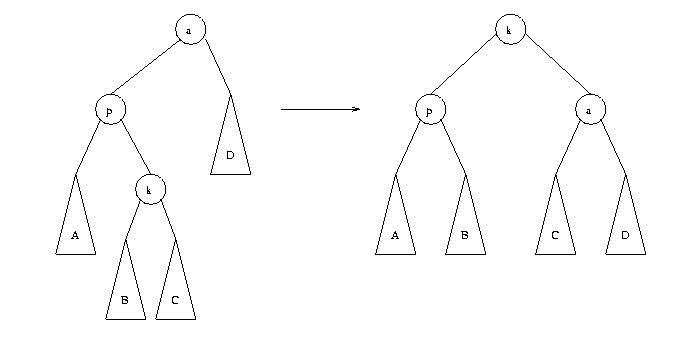
\includegraphics[width=0.7\textwidth]{rotacion_zig_zag.png}
            \caption*{Diagrama de una rotación zig-zag}
        \end{figure}
        \begin{figure}[H]
            \centering
            \textbf{Rotación Zig-Zig}\par\medskip
            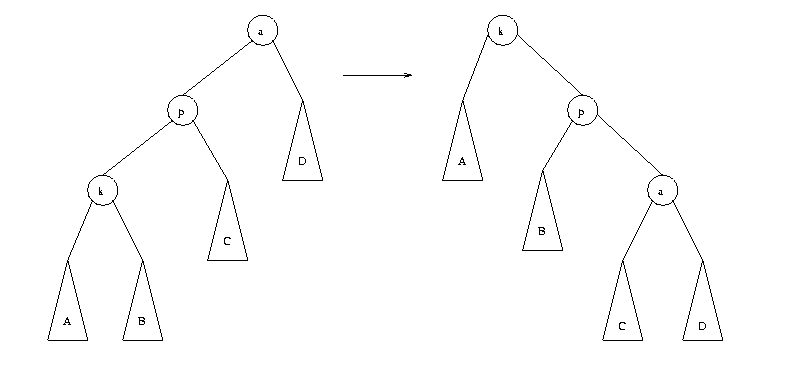
\includegraphics[width=0.7\textwidth]{rotacion_zig_zig.png}
            \caption*{Diagrama de una rotación zig-zig}
        \end{figure}
        Estas rotaciones se aplican hasta mover el elemento hasta la raíz.
\end{itemize}

La inserción se realiza como en cualquier otro ABB, solo que se realizan las operaciones de rotación para que el elemento quede en la raíz. Para borrar un elemento, primero se lo busca, lo cual lo deja en la raíz, luego se busca el mayor elemento del subárbol izquierdo, que pasa a ser la nueva raíz, como ese elemento era un antecesor inmediato, no tiene subárbol derecho, así que el subárbol derecho original queda como nuevo subárbol derecho.

Los splay trees resultan más simples de implementar que los árboles balanceados, y no tienen requerimientos de memoria adicionales. Si bien no se puede garantizar $\BigO{\log{n}}$ por operación, una secuencia de $m$ operaciones tendrá tiempo $\BigO{\log{m\log{n}}}$ (tiene tiempo $\BigO{\log{n}}$ amortizado).

\subsection{Análisis amortizado}

El análisis \textit{amortizado} permite asegurar garantías de la complejidad de secuencias de operaciones, en lugar de una única ejecución. Existen 2 mecanismos para demostrar complejidades amortizadas: el método del banquero y el método de potenciales.

% Lo demás no lo explica suficiente como para escribirlo

\appendix

\section{Apéndice -- Tablas}

\label{table-dict-complexities}

\end{document}
